%%%%%%%%%%%%%%%%%%%%%%%%%%%%%%%%%%%%%%%%%%%%%%%%%%%%%%%%%%%%%%%%%%%%%%%%%%%%%%%%
%2345678901234567890123456789012345678901234567890123456789012345678901234567890
%        1         2         3         4         5         6         7         8

\documentclass[letterpaper, 10 pt, conference]{ieeeconf}  % Comment this line out if you need a4paper

%\documentclass[a4paper, 10pt, conference]{ieeeconf}      % Use this line for a4 paper

\IEEEoverridecommandlockouts                              % This command is only needed if 
                                                          % you want to use the \thanks command

\overrideIEEEmargins                                      % Needed to meet printer requirements.

%In case you encounter the following error:
%Error 1010 The PDF file may be corrupt (unable to open PDF file) OR
%Error 1000 An error occurred while parsing a contents stream. Unable to analyze the PDF file.
%This is a known problem with pdfLaTeX conversion filter. The file cannot be opened with acrobat reader
%Please use one of the alternatives below to circumvent this error by uncommenting one or the other
%\pdfobjcompresslevel=0
%\pdfminorversion=4

% See the \addtolength command later in the file to balance the column lengths
% on the last page of the document

% The following packages can be found on http:\\www.ctan.org
\usepackage{graphicx} % for pdf, bitmapped graphics files
%\usepackage{epsfig} % for postscript graphics files
%\usepackage{mathptmx} % assumes new font selection scheme installed
%\usepackage{times} % assumes new font selection scheme installed
%\usepackage{amsmath} % assumes amsmath package installed
%\usepackage{amssymb}  % assumes amsmath package installed

\title{\LARGE \bf
From Evaluating to Teaching:\\
Rewards and Challenges of Human Control for Learning Robots
}


\author{Emmanuel Senft, S\'{e}verin Lemaignan, Paul Baxter and Tony Belpaeme% <-this % stops a space
%\thanks{*This work was not supported by any organization}% <-this % stops a space
%\thanks{$^{1}$Albert Author is with Faculty of Electrical Engineering, Mathematics and Computer Science,
%        University of Twente, 7500 AE Enschede, The Netherlands
%        {\tt\small albert.author@papercept.net}}%
%\thanks{$^{2}$Bernard D. Researcheris with the Department of Electrical Engineering, Wright State University,
%        Dayton, OH 45435, USA
%        {\tt\small b.d.researcher@ieee.org}}%
}


\begin{document}



\maketitle
\thispagestyle{empty}
\pagestyle{empty}


%%%%%%%%%%%%%%%%%%%%%%%%%%%%%%%%%%%%%%%%%%%%%%%%%%%%%%%%%%%%%%%%%%%%%%%%%%%%%%%%
\begin{abstract}
Keeping a human in a robot learning loop can provide many advantages to improve the learning process. However, most of these improvements are only available when the human teacher is totally in control of the robot's behaviour, not a simple evaluator. 
advantages

challenges

limitations

\end{abstract}


%%%%%%%%%%%%%%%%%%%%%%%%%%%%%%%%%%%%%%%%%%%%%%%%%%%%%%%%%%%%%%%%%%%%%%%%%%%%%%%%
\section{INTRODUCTION}

Interactive Machine Learning (IML) \cite{fails2003interactive,amershi2014power} differs from Classical Machine Learning in the fact that the learning process is not one single monolithic step leading to a static classifier or robot behaviour. IML relies on a series of small steps of learning progressively leading to a complete and autonomous system. Additionally, IML makes use of humans in the learning loop, to direct the learning process, making it at the same time faster, more adequate to the task and more efficient.

IML can take two form: human supported classifiers or human guided learning agent. A classical example of the first category is Active Learning, a form of learning giving to the learning the opportunity to take a more active stance in the process, asking questions and querying labels from an oracle, often a human being \cite{settles2012active}. The second category relates to agents learning to interact in an environment and profiting from humans inputs improving the learning process. In this case, the learner is not in control of the datapoints it has to classify as those come directly form the environment, in fact, the agent is provided with inputs form the environment and has to select a correct action at each time step.

This work is focused on the second category, agents learning from human supervision to interact in an environment. 

\begin{figure}[ht]
	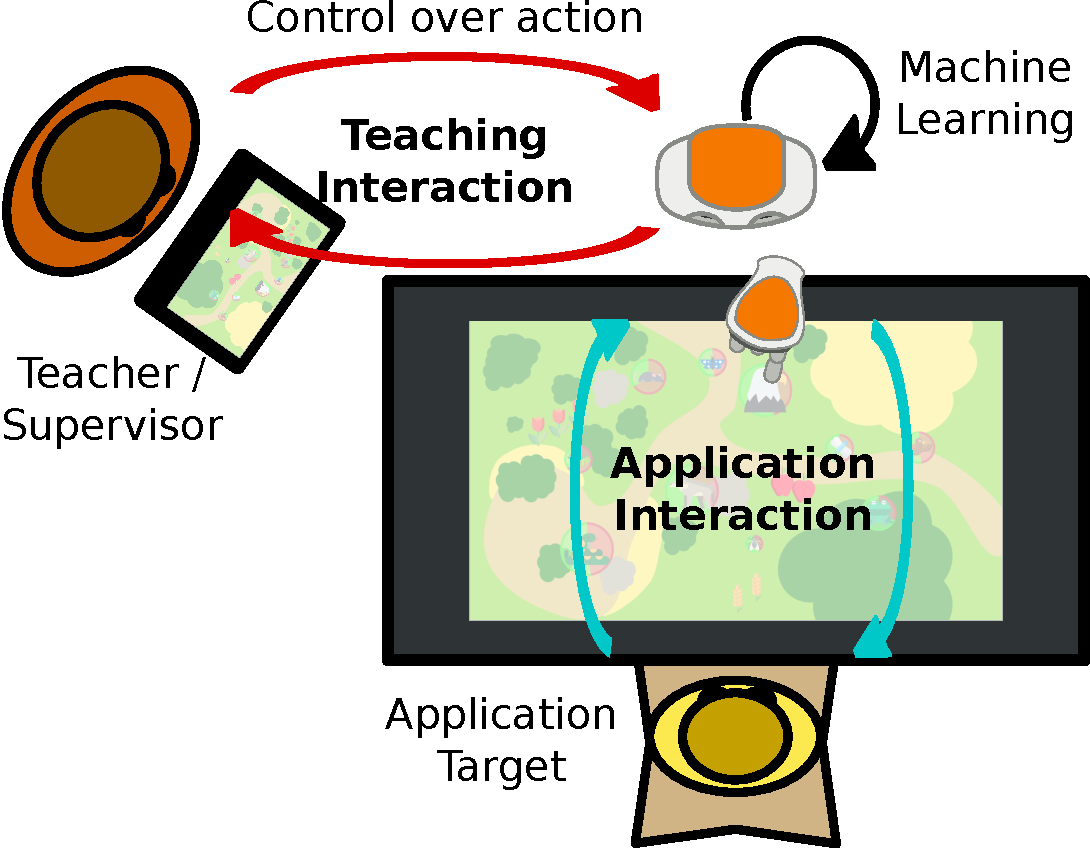
\includegraphics[width=.8\linewidth]{setup.pdf}
	\centering
	\caption{Example of a human teaching a robot to interact with a child in an educational scenario.}
	\label{fig:frame}
\end{figure}


What is iml and why it's amazing

how could it be applied to agents learning to interact 
quickly pass active learning 

\cite{fails2003interactive,amershi2014power} 

human rewards

\cite{thomaz2008teachable}
\cite{loftin2016learning}
\cite{macglashan2017interactive}
\cite{munzer2017efficient}
but could be much better
\cite{senft2017supervised} 

\cite{senft2015sparc}

\section{Advantages of Human Control}

Robot learning possess a unique opportunity compared to human learning in that the teacher can be fully in control of the learner's behaviour. This control over the learner provides many opportunities for agents learning from humans. Instead of simply labelling the agent's action, as in methods such as TAMER \cite{knox2009interactively}, the teacher can take over the learning demonstrating an efficient behaviour. Methods such as Learning from Demonstration (LfD) \cite{argall2009survey,billard2008robot} leverage this opportunity often in manipulation scenario to reach quickly an efficient behaviour. However, this human control can be pushed 

\subsection{Safety}

\subsection{Generalisation}

\subsection{Speed}

\subsection{Trust}

\section{Challenges}

\subsection{Interface}

\subsection{Human Time}

\subsection{Human Limits}

\section{Discussion}

\section*{ACKNOWLEDGMENT}

This work was supported by the EU FP7 DREAM project (grant no.  611391).



%\begin{thebibliography}{99}
\bibliographystyle{IEEEtran}
\bibliography{Bib.bib}

%\end{thebibliography}




\end{document}
